\documentclass{article}[18pt]
\ProvidesPackage{format}
%Page setup
\usepackage[utf8]{inputenc}
\usepackage[margin=0.7in]{geometry}
\usepackage{parselines} 
\usepackage[english]{babel}
\usepackage{fancyhdr}
\usepackage{titlesec}
\hyphenpenalty=10000

\pagestyle{fancy}
\fancyhf{}
\rhead{Sam Robbins}
\rfoot{Page \thepage}

%Characters
\usepackage{amsmath}
\usepackage{amssymb}
\usepackage{gensymb}
\newcommand{\R}{\mathbb{R}}

%Diagrams
\usepackage{pgfplots}
\usepackage{graphicx}
\usepackage{tabularx}
\usepackage{relsize}
\pgfplotsset{width=10cm,compat=1.9}
\usepackage{float}

%Length Setting
\titlespacing\section{0pt}{14pt plus 4pt minus 2pt}{0pt plus 2pt minus 2pt}
\newlength\tindent
\setlength{\tindent}{\parindent}
\setlength{\parindent}{0pt}
\renewcommand{\indent}{\hspace*{\tindent}}

%Programming Font
\usepackage{courier}
\usepackage{listings}
\usepackage{pxfonts}

%Lists
\usepackage{enumerate}
\usepackage{enumitem}

% Networks Macro
\usepackage{tikz}


% Commands for files converted using pandoc
\providecommand{\tightlist}{%
	\setlength{\itemsep}{0pt}\setlength{\parskip}{0pt}}
\usepackage{hyperref}

% Get nice commands for floor and ceil
\usepackage{mathtools}
\DeclarePairedDelimiter{\ceil}{\lceil}{\rceil}
\DeclarePairedDelimiter{\floor}{\lfloor}{\rfloor}

% Allow itemize to go up to 20 levels deep (just change the number if you need more you madman)
\usepackage{enumitem}
\setlistdepth{20}
\renewlist{itemize}{itemize}{20}

% initially, use dots for all levels
\setlist[itemize]{label=$\cdot$}

% customize the first 3 levels
\setlist[itemize,1]{label=\textbullet}
\setlist[itemize,2]{label=--}
\setlist[itemize,3]{label=*}

% Definition and Important Stuff
% Important stuff
\usepackage[framemethod=TikZ]{mdframed}

\newcounter{theo}[section]\setcounter{theo}{0}
\renewcommand{\thetheo}{\arabic{section}.\arabic{theo}}
\newenvironment{important}[1][]{%
	\refstepcounter{theo}%
	\ifstrempty{#1}%
	{\mdfsetup{%
			frametitle={%
				\tikz[baseline=(current bounding box.east),outer sep=0pt]
				\node[anchor=east,rectangle,fill=red!50]
				{\strut Important};}}
	}%
	{\mdfsetup{%
			frametitle={%
				\tikz[baseline=(current bounding box.east),outer sep=0pt]
				\node[anchor=east,rectangle,fill=red!50]
				{\strut Important:~#1};}}%
	}%
	\mdfsetup{innertopmargin=10pt,linecolor=red!50,%
		linewidth=2pt,topline=true,%
		frametitleaboveskip=\dimexpr-\ht\strutbox\relax
	}
	\begin{mdframed}[]\relax%
		\centering
		}{\end{mdframed}}



\newcounter{lem}[section]\setcounter{lem}{0}
\renewcommand{\thelem}{\arabic{section}.\arabic{lem}}
\newenvironment{defin}[1][]{%
	\refstepcounter{lem}%
	\ifstrempty{#1}%
	{\mdfsetup{%
			frametitle={%
				\tikz[baseline=(current bounding box.east),outer sep=0pt]
				\node[anchor=east,rectangle,fill=blue!20]
				{\strut Definition};}}
	}%
	{\mdfsetup{%
			frametitle={%
				\tikz[baseline=(current bounding box.east),outer sep=0pt]
				\node[anchor=east,rectangle,fill=blue!20]
				{\strut Definition:~#1};}}%
	}%
	\mdfsetup{innertopmargin=10pt,linecolor=blue!20,%
		linewidth=2pt,topline=true,%
		frametitleaboveskip=\dimexpr-\ht\strutbox\relax
	}
	\begin{mdframed}[]\relax%
		\centering
		}{\end{mdframed}}
\lhead{Programming Paradigms - Functional Programming}
\usepackage{minted}
\usepackage{enumitem}
\usepackage{pifont}
\setminted{tabsize=2}
\newcommand{\xmark}{\ding{55}}%
\begin{document}
\begin{center}
\underline{\huge Introduction}
\end{center}
\section{Computing n!}
\textit{Imperative style:}
\begin{minted}{python}
for i in range(1, n+1):
	factorial=factorial * i
\end{minted}
\textit{Functional Style}
\begin{minted}{python}
def factorial(n):
	if n==1:
		return 1
	else:
		return n*factorial(n-1)
\end{minted}
\section{What is a functional language}
A style of programming where the building block of computation is an application to arguments. 
\section{Side effects}
\textbf{Side effect} - Modify some (internal/hidden) state as well as returning a value\\
\\
An example of this:\\
\texttt{y1=f(1)}\\
\texttt{y2=f(2)}\\
\\
You would expect \texttt{y1==y2}, however if f has an internal state that affects the answer this will not be true
\begin{minted}{python}
state=0
def f(n):
	global state
	state +=1
	return n+ state
	
print(f(1))=> "2"
print(f(1))=> "3"
\end{minted}
\section{A functional approach}
\begin{itemize}
	\item Forbid variable assignment and side effects in the language "pure functional"
	\item [$\checkmark$] Makes reasoning about code simpler (for humans and compilers)
	\item [\xmark] A new programming paradigm: takes some time to get used to
\end{itemize}
\section{Why programming languages}
\subsection{Abstracting from the machine}
$$b=a+3$$
\begin{minted}{gas}
mov addr_a, reg1 ##Load address of a into reg1
add 3, reg1, reg2 ## add 3 to reg1 and write into reg2 
mov reg2, addr_b ## write reg2 to address of b
\end{minted}
\begin{itemize}
	\item [$\checkmark$] Explicit about what is going on
	\item [\xmark] Obfuscates algorithm from implementation
	\item [\xmark] Not portable (would need different instructions for different hardware e.g. different registers)
	\item [\xmark] Not easy to modify
	\item [\xmark] Not succinct
\end{itemize}
\subsection{Programming languages}
\begin{itemize}
	\item Allow writing code to an abstract machine model
	\item A translator of some kind (perhaps a compiler) transforms this code into something that executes on some hardware (sometimes this hardware is a virtual machine)
	\item Some virtual machines are "hybrid": they do just-in-time compilation
	\item The Haskell distribution we will use has both Compiler and Interpreter mode
\end{itemize}
\begin{center}
	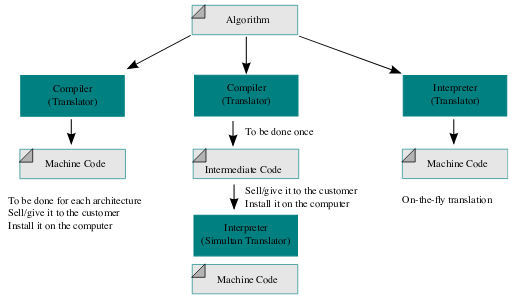
\includegraphics[scale=0.7]{Compiler}
\end{center}
\begin{itemize}
	\item Micro-architecture just reads an instruction stream
	\item Note easy to program complex algorithms in such a "language" so use abstractions leading to high level languages
	\item Features driven by programming paradigm considerations, domain knowledge, wanting to target particular hardware...
	\item Compiler or interpreter maps this language onto machine instructions
	\item Therefore we need a formal specification 
\end{itemize}
\section{Example}
\begin{minted}{haskell}
filter:: (a -> Bool) -> [a] -> [a]
filter p [] = []
filter p (x:xs)
	| p x 	= x: filter p xs
	| otherwise	= filter p xs
\end{minted}
\begin{itemize}
	\item Higher order
	\item Polymorphic (works for all types a) (functions that take functions as parameters)
	\item Function defined with recursion and pattern matching
\end{itemize}
\section{Syntax and Semantics}
\textbf{Syntax} - What are valid sentences (expressions) in a language?\\
\textbf{Semantics} - What do these valid sentences (expressions) mean?
\section{Naming Requirements}
\begin{itemize}
	\item Can have characters in function names, for example \texttt{x'}
	\item s at the end to show a list
	\item lowercase letter to start
\end{itemize}
\section{Comments}
\begin{minted}{haskell}
-- Comment like this
{- Or like this if you have multiple 
lines -}
\end{minted}


\end{document}